\documentclass[12pt]{report}

\usepackage{minted}
\usepackage{fullpage}
\usepackage{amsmath,amssymb,bm,upgreek,mathrsfs}
\usepackage{algorithmic,algorithm}
\usepackage{graphicx,subcaption}
\usepackage{setspace}
\usepackage{color}
\usepackage{multirow}
\usepackage{alltt}
\usepackage{cancel}
\usepackage{listings}

\doublespacing

\DeclareMathOperator*{\argmax}{arg\,max}
\DeclareMathOperator*{\argmin}{arg\,min}

\newcommand{\N}{\mathcal{N}} \newcommand{\U}{\mathcal{U}}
\newcommand{\Poi}{{\text Poisson}} \newcommand{\Exp}{{\text Exp}}
\newcommand{\G}{\mathcal{G}} \newcommand{\Ber}{{\text Bern}}
\newcommand{\Lap}{{\text Laplace}} \newcommand{\btheta}{\boldsymbol{\theta}}
\newcommand{\bSigma}{\boldsymbol{\Sigma}}

\newcommand{\E}[1]{\mathbb{E}[#1]}
\newcommand{\Cov}[2]{\mathbb{C}\mathrm{ov}(#1,#2)}

\def\*#1{\mathbf{#1}} \newcommand*{\V}[1]{\mathbf{#1}}

%%%%%%%%%%%%%%%%%%%%%%%%%%%%%%%%%%%%%%%%%%%%%%%%%%%%%%%%%%%%%%%%%%%%%%

\begin{document}

\centerline{\it CS 480 HW \#2}

\begin{enumerate}

\item[1.] Effort level.

\item[a.] The homework took me 12 hours.
\item[b.] N\textbackslash A
\item[c.] Used ChatGPT as a tool to look up syntax and documentation for
  Scikit-learn and related machine learning libraries.

\item[2.] Paired t-test.

\item[a.] 95\% confidence interval.

  Below, I provide the code for constructing the 95\% confidence interval.
\begin{minted}{python}
from scipy.stats import norm, ttest_rel, t
import numpy as np
# 2a
f = open('./data.txt', 'r')
A = []
B = []
for line in f:
  line = line.strip().split()
A.append(float(line[0]))
B.append(float(line[1]))

a = np.array(A)
b = np.array(B)

mean_a = np.mean(a)
mean_b = np.mean(b)

std_a = np.std(a,ddof=1)
std_b = np.std(b,ddof=1)

n = len(a)
print(n)
alpha = 0.05
tci_a = t.interval(1-alpha, n-1, mean_a, std_a/np.sqrt(n))
tci_b = t.interval(1-alpha, n-1, mean_b, std_b/np.sqrt(n))

print('Algorithm A CI:')
print(tci_a)
print()
print('Algorithm B CI:')
print(tci_b)
\end{minted}

The output of the Python script is reported.

Algorithm A CI:
(np.float64(2.3434452353035717), np.float64(3.8232214313630952))

Algorithm B CI:
(np.float64(1.5268346967576174), np.float64(2.9731653032423826))

Based on the reporting, we can say that two confidence intervals overlap.
However, we cannot say that one algorithm is better than the other since they do
indeed overlap, and a paired t-test is required to determine if one is better
than the other in a statistically meaningful way.
\item[b.] Two-sided paired t-test for null-hypothesis.

  The code for computing the t-test is as follows.
\begin{minted}{python}
print(ttest_rel(a, b).confidence_interval)
\end{minted}
This outputs the following result.

TtestResult(statistic=np.float64(2.277867258047101),
pvalue=np.float64(0.043699584804600185), df=np.int64(11))

Since the standard t-distribution with 11 degrees of freedom and 95\% confidence
is known to be 2.201, and so interval being [-2.201, 2.201], we know that our
t-stat of 2.278 goes out of this interval, so we are safe to reject the null
hypothesis and say that one algorithm has a statistically difference in
performance compared to the other. From this experiment, we can see that
two-sided paired t-test to find a statistically significant difference
between two algorithms is concrete and deterministic while comparing two
separate confidence intervals does not really allow us to conclude anything,
even if they do overlap as they did in this case.

\item[c.] Report p-value for testing done in b.

  The p-value as reported in part b is 0.044. We know that the two algorithms
  are statistically different because our p-value falls below our 0.05
  significance threshold. This is another way to determine if the results of two
  models are statistically different from each other.
\item[d.] Describe pseudocode for bootstrapping method for this problem.

  The pseudocode for bootstrapping is as follows.

  Obtain F1 score for each fold.

  Sort them in increasing order.

  Compute the top .25 quantile.

  Compute the bottom .25 quantile.

  The CI is [F1 - top quantile, F1 + lower quantile]

\item[e.] Implement and perform bootstrapping paired test with computed p-value.

  \newpage
\item[3.] Linear regression.

\item[a.] Plot year versus ice days.

  Below, I provide the plot of annual ice cover days for Lake Mendota and Lake
  Monona.

  \begin{figure}[H]
    \centering \fbox{
      \begin{minipage}{.98\linewidth}
        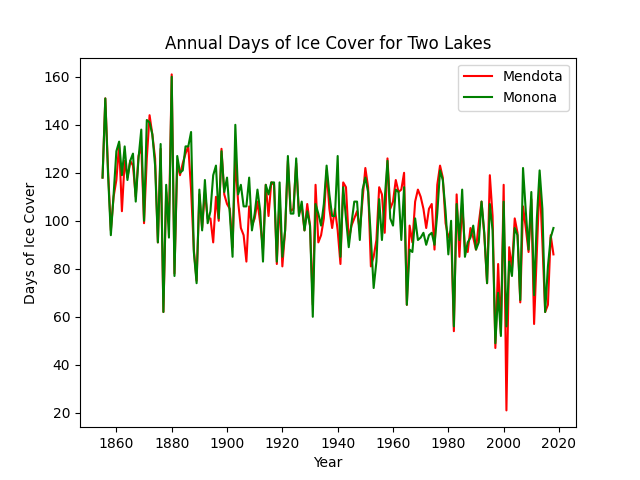
\includegraphics[width=\linewidth]{p2/ice_cover.png}
        \caption{Plot of annual ice cover days for Lake Mendota (red) and Lake
          Monona (green) using Python.}
        \label{fig:3a}
      \end{minipage}}
  \end{figure}

  Below, I provide the plot of the difference in annual days of ice cover
  between Lake Monona and Lake Mendota (Lake Monona - Lake Mendota).

  \begin{figure}[H]
    \centering \fbox{
      \begin{minipage}{.98\linewidth}
        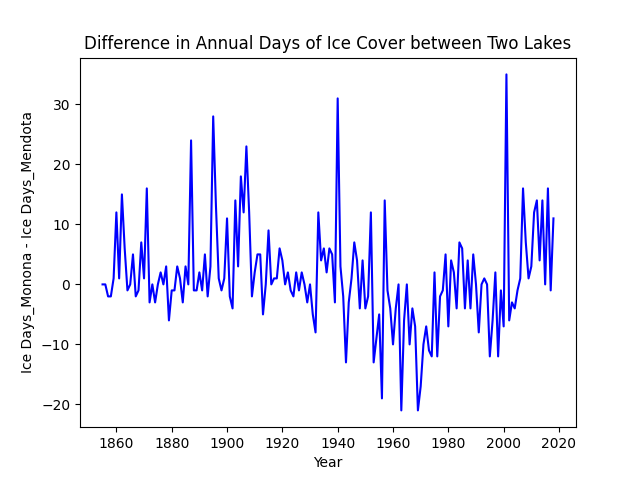
\includegraphics[width=\linewidth]{p2/diff.png}
        \caption{Plot of the difference in annual days of ice cover between Lake
        Monona and Lake Mendota using Python.}
        \label{fig:3b}
      \end{minipage}}
  \end{figure}

  Below is the Python script used to generate the two plots.
\begin{minted}{python}
import pandas as pd
import matplotlib.pyplot as plt
import numpy as np

# load in csv data
col = 'Days of Ice Cover'

mendota_df =
pd.read_csv('mendota.csv')
.loc[5:175].dropna(subset=[col]).iloc[::-1].reset_index(drop=True)

monona_df =
pd.read_csv('monona.csv')
.loc[6:176].dropna(subset=[col]).iloc[::-1].reset_index(drop=True)

# 3a
plt.figure(1)
plt.plot([x for x in range(1855,2019)],mendota_df[col], color='red')
plt.plot([x for x in range(1855,2019)],monona_df[col], color='green')
plt.xlabel('Year')
plt.ylabel(col)
plt.title('Annual Days of Ice Cover for Two Lakes')
plt.legend(['Mendota', 'Monona'])
plt.savefig('ice_cover.png')
plt.show()

diff = []
for i,j in zip(monona_df[col],mendota_df[col]):
    diff.append(i-j)

plt.figure(2)
plt.plot([x for x in range(1855,2019)],diff, color='blue')
plt.xlabel('Year')
plt.ylabel('Ice Days_Monona - Ice Days_Mendota')
plt.title('Difference in Annual Days of Ice Cover between Two Lakes')
plt.savefig('diff.png')
plt.show()
\end{minted}

\item[b.] Split the datasets into training and testing. Compute std and mean for
  the two lakes respetively.

  The results are as follows.

  Mendota Mean:
  107.19

  Mendota STD:
  16.74

  Monona Mean:
  108.48

  Monona STD:
  18.12

  Below is the Python script used to compute the means and STDs.
\begin{minted}{python}
# 3b
split = mendota_df.index[mendota_df['Winter'] == '1970-71'].tolist()[0] + 1
mendota_df_train = mendota_df.iloc[:split]
mendota_df_test = mendota_df.iloc[split:]
split = monona_df.index[monona_df['Winter'] == '1970-71'].tolist()[0] + 1
monona_df_train = monona_df.iloc[:split]
monona_df_test = monona_df.iloc[split:]

mendota_a = np.array(mendota_df_train[col])
monona_a = np.array(monona_df_train[col])

print('Mendota Mean:')
print(np.mean(mendota_a))
print('Mendota STD:')
print(np.std(mendota_a,ddof=1))
print()
print('Monona Mean:')
print(np.mean(monona_a))
print('Monona STD:')
print(np.std(monona_a,ddof=1))
\end{minted}

\item[c.] Using training sets, train a linear regression model.

  Scikit-learn in Python was used for this section.

  Below I provide the Python script for training a linear regression model.
\begin{minted}{python}
# 3c
from sklearn.linear_model import LinearRegression
from sklearn.model_selection import train_test_split
from sklearn.metrics import mean_squared_error

lr = LinearRegression()
monona_df_train['ones'] = 1
monona_df_test['ones'] = 1
lr.fit(monona_df_train[['ones','Winter',col]], mendota_df_train[[col]])
mendota_pred = lr.predict(monona_df_test[['ones','Winter', col]])

weights = lr.coef_
print(weights)
intercept = lr.intercept_
print(intercept)
\end{minted}

The results are as follows:

Feature weights: [[0., 0.04122457, 0.85295064]]

Intercept:[-64.1827663]

These are the relevant outputs of the Scikit-learn LinearRegression model. One
thing to note is that although we are trying to get an intercept in our OLS
solution by modeling our features as (1, x, $y_{monona}$), the LinerRegression
model in Scikit-learn does not seem to care about an artificial `1' appended to
the feature vector and will in fact produce the same result without the `1'
column, so we can get away with just (x, $y_{monona}$). As reported above, the
feature weights which represent $(B_0, B_1,B_2)$ omits the $B_0$ value; probably
because it ignores a column of 1's like I mentioned. Instead, it will report our
$B_0$ (which is our intercept) in its own category called `intercept'.

\item[d.] Mean squared error on the test set.

  Below, I provide the Python script to compute the MSE of our predicted values
  from our Scikit-learn LinearRegression model. The computation of MSE is also
  provided in the Scikit-learn library.
\begin{minted}{python}
# 3d
mse = mean_squared_error(mendota_df_test[[col]], mendota_pred)
print(mse)
\end{minted}

The result of this script is reported below.

Mean sqaure error: 124.26409483990123

This is a fairly nice MSE since it is the square of the mean error value. It
means our linear regression model is on average about 11 days off the mark every
year.

\item[e.] Train a linear regression model using Monona.

  Below, I provide the Python script for retraining our linear regression model
  on our new feature vector which just omits $y_{monona}$.
\begin{minted}{python}
# 3e

lr2 = LinearRegression()
lr2.fit(monona_df_train[['ones', 'Winter']],mendota_df_train[[col]])
mendota_pred2 = lr2.predict(monona_df_test[['ones', 'Winter']])
mse2 = mean_squared_error(mendota_df_test[[col]], mendota_pred2)

weights2 = lr2.coef_
intercept2 = lr2.intercept_

print('Feature weights: ' + str(weights2))
print('Intercept:' + str(intercept2))
print('Mean sqaure error: ' + str(mse2))
\end{minted}

I report the newly trained linear model below.

Feature weights: [[ 0., -0.15629877]]

Intercept:[406.11105985]

Mean sqaure error: 418.14436543672855

As seen above, the MSE is much higher when the linear model only has the year
and cannot reference $y_{monona}$ in order to predict $y_{mendota}$. This
intuitively makes sense. Remember that the first element of the feature weights
which should be intercept is simply reported in a separate variable called
`intercept' in Scikit-learn's LinerRegression model.

  \begin{itemize}
  \item[i.] Interpret the sign of $\gamma_1$.

    $\gamma_1$ can be interpreted as the slope of our x variable. Since it is
    negative, we can say that it derived a directly negative correlation between
    the year and the number of ice days. In other words, as the years go by and
    `increases', the number of ices days decrease. Even more simply put, our
    model predict a warming trend.
  \item[ii.] Assessing a viewpoint formed from the model.

    The stated viewpoint could be wrong because looking at our model again, it
    can be seen that the strongest weight $B_2=0.85$ is much greater than the
    $B_1=0.04$ that the analysts are referring to. $B_2$ is the weigh of feature
    $y_{monona}$ on label $y_{mendota}$ and since they have a strong correlation
    to each other and are trending downwards together, there is little weight on
    $B_1$ which is the number of years since feature $y_{monona}$ is doing all
    the `heavy lifting'. In fact, it is more accurate to say that $B_1$ is
    zero-ish weight, and it was a coincidence that it happened to be barely
    positive as a part of the OLS solution.
  \end{itemize}

\item[4.] Maximum likelihood estimation for linear regression.

\item[a.] Likelihood of the ith data point.

  $Laplace(\mu ,b) \rightarrow f(z|\mu , b) = \frac{1}{2b}e^{-\frac{|z-u|}{b}}$

  $Laplace(w^Tx,1) \rightarrow f(z|w^Tx, 1) = \frac{1}{2}e^{-|z-u|}$

  $P(y_i|x_iw)=f(y_i|w^Tx_i,1)$

  $= \frac{1}{2}e^{-|y_i-w^Tx_i|}$
\item[b.] Log-likelihood of the dataset.

  $L = P(y_1...,y_n|x_1,...,x_n,w)$

  $=\prod_{i=1}^{n}P(y_i|x_i,w)$

  $=\prod_{i=1}^{n}(\frac{1}{2}e^{-|y_i-w^Tx_i|})$

  $\log(L) = \log(\prod_{i=1}^{n}(\frac{1}{2}e^{-|y_i-w^Tx_i|}))$

  $=\sum_{i=1}^{n}\log(\frac{1}{2}e^{-|y_i-w^Tx_i|})$

  $=n\log(\frac{1}{2})+\sum_{i=1}^{n}\log(e^{-|y_i-w^Tx_i|})$

  $=n\log(\frac{1}{2})+\sum_{i=1}^{n}(-|y_i-w^Tx_i|)$

  $=n\log(\frac{1}{2})-\sum_{i=1}^{n}|y_i-w^Tx_i|$

  $w^{MLE}=\argmax_w\sum_{i=1}^{n}(\log(\frac{1}{2}) - |y_i-w^Tx_i|)$

  $w^{MLE}=\argmin_w\sum_{i=1}^{n}|y_i-w^Tx_i|$

  From our derivation, the optimization problem is to find the value of $w$ that
  would minimize $\sum_{i=1}^{n}|y_i-w^Tx_i|$.

  This is not equivalent to the least squares problem because our derivation
  above shows we are minimizing the residuals of the points to a line which is
  consistent with our study of linear regression. In least squares however, you
  want to take the zero derivative of a convex, quadratic function in order to
  find the global minimum, and the derived $w^{MLE}$ from finding this is, in
  general, not the same problem as minimizing residuals.

\item[c.] Maximum likelihood estimator $w$ under the above model.

  $w^{MLE}=\argmin_w\sum_{i=1}^{n}|y_i-w^Tx_i|$

  $w^{MLE}=\min_w(|3-w(1)|+|5-w(1)|+|6-w(1)|)$

  $w^{MLE}=\min_w(|3-w|+|5-w|+|6-w|)$

  Then, let $f(w) = |3-w|+|5-w|+|6-w|$. Below, I provide the plot of $f(w)$.

  \begin{figure}[H]
    \centering \fbox{
    \begin{minipage}{.98\linewidth}
      \includegraphics[width=\linewidth]{Screenshot 2024-10-03 at 1.00.00 PM.png}
      \caption{Plot of $f(w)$ in MATLAB. The clicked point at (5,3) is the
        global minimum of $f(w)$.}
      \label{fig:4c}
    \end{minipage}}
  \end{figure}

  From the plot above, we can see that the function $f(w)$ is minimized when
  $w=5$, so we have $w^{MLE}=\min_w(|3-w|+|5-w|+|6-w|) = 5$.
% \item[B.] Making a world coordinate system.
%   Below in Figure 4, I provide the world coordinate system for the image provided
%   for hw03.

%   \begin{figure}[H]
%     \centering \fbox{
%       \begin{minipage}{.98\linewidth}
%         \includegraphics[width=\linewidth]{IMG_0862.jpeg}
%         \caption{World coordinate system for provided image for hw03. The X, Y,
%           and Z axes are clearly labeled, and the direction of the axes' arrows
%           indicate in which direction they grow. 15 blue points have been
%           selected for this experiement as shown, and their (X,Y,Z) coordinates
%           are labeled in yellow.}
%         \label{fig:b1}
%       \end{minipage}}
%   \end{figure}

%   These 15 blue world coordinate points in Figure 4 will be used for Part C to
%   compare how two cameras map these 3D world coordinates to 2D. The files
%   world\_coords.txt and image\_coords.txt have also been provided in this
%   submission for Part C. The world coordinates of the points are as they are in
%   Figure 4, and the image coordinates (X, Y) were obtained using the
%   `datacursormode on' feature in MATLAB and manually clicking on the labeled
%   blue points.

% \item[C.] Analyzing how a camera matrix maps points from 3D to 2D.

%   Below in Figure 5, I provide the visual representation of our clicked world
%   coordinates along with the two camera estimates of our world coordinates.

%   \begin{figure}[H]
%     \centering \fbox{
%       \begin{minipage}{.98\linewidth}
%         \includegraphics[width=\linewidth]{Screenshot 2024-09-29 at 11.19.16 PM.png}
%         \caption{The red clicked points are our world coordinates from Figure 4
%           moved onto this black canvas to compare to our first (green) and
%           second (blue) camera estimates. Produced in MATLAB.}
%         \label{fig:c1}
%       \end{minipage}}
%   \end{figure}

%   In Figure 5 above, we can see that both the first and camera estimates are
%   visually close to our red clicked points. One thing to note when plotting the
%   estimates was to flip the X and Y coordinates generated from the given camera
%   matrices which we explored the reason for in Part A.

%   The RMSE of the distance between the camera estaimte point and the actual
%   clicked point was calculated for both cameras in MATLAB. Again, when
%   calculating the distsances between points, we have to flip the coordinates
%   generated from the camera matrices, or flip the image coordinates of the world
%   coordinates. The key thing is to be consistent with our coordinate system
%   (either work in X vs Y values or work with indices of a matrix). The RMSEs are
%   as follows:

%   $RMSE_{camera1}=23.9$

%   $RMSE_{camera2}=40.7$

%   The RMSE of the camera estimated points and actual world coordinate points is
%   also known as the re-projection error as stated in the homework. From the
%   reported RMSEs of the cameras, the first camera is better quantitatively
%   speaking, and from scrutinizing Figure 5, one can see that the first camera
%   (green) points are closer to the clicked (red) points than the second (blue)
%   camera points on average.

%   Thus, the first camera's matrix is more accurate.

\end{enumerate}

\end{document}
